\chapter{Introduction}
\label{c:introduction}

Particle physics research over the last century or so has provided us with our current basic understanding of
the fundamental particles that have made up the universe since its origin, and their interactions with each
other. This is summarised by the Standard Model (SM) of particle physics, which has been developed
incrementally in recent decades and has stood up well to scientific scrutiny. The Large Hadron Collider (LHC)
at the Organisation Europ\'{e}enne pour la Recherche Nucl\'{e}aire (CERN) near the Swiss city of Geneva
(Figure~\ref{fig:LHC_map}) was constructed with the aim of investigating the SM. Areas of current interest
such as the electroweak symmetry breaking, the Higgs mechanism and physics beyond the SM (BSM) such
as supersymmetry (explained in further detail in Section~\ref{c:the_standard_model_and_top_physics}), require
the acceleration of particles to high energies (of the order of several TeV). The start of data-taking from proton-proton collisions at the
LHC in 2009 ushered in a new era in terms of energies at particle colliders, taking over as the highest energy
particle collider from the TeVatron at Fermilab. In 2010 and 2011 the LHC collected data at a centre of mass
energy of 7~\TeV (5.1~\fbinv), followed by 8~\TeV (21.8~\fbinv) in 2012 and currently in 2015 after Long
Shutdown 1 at 13~\TeV.

The Compact Muon Solenoid (CMS) general-purpose detector is one of four detectors located around the LHC (the
others being ATLAS, LHCb and ALICE), approximately 100~m below ground level. The geographical site and
location of the various experiments are shown in Figure~\ref{fig:LHC_map}.

\begin{figure}[hbtp]
   \centering
     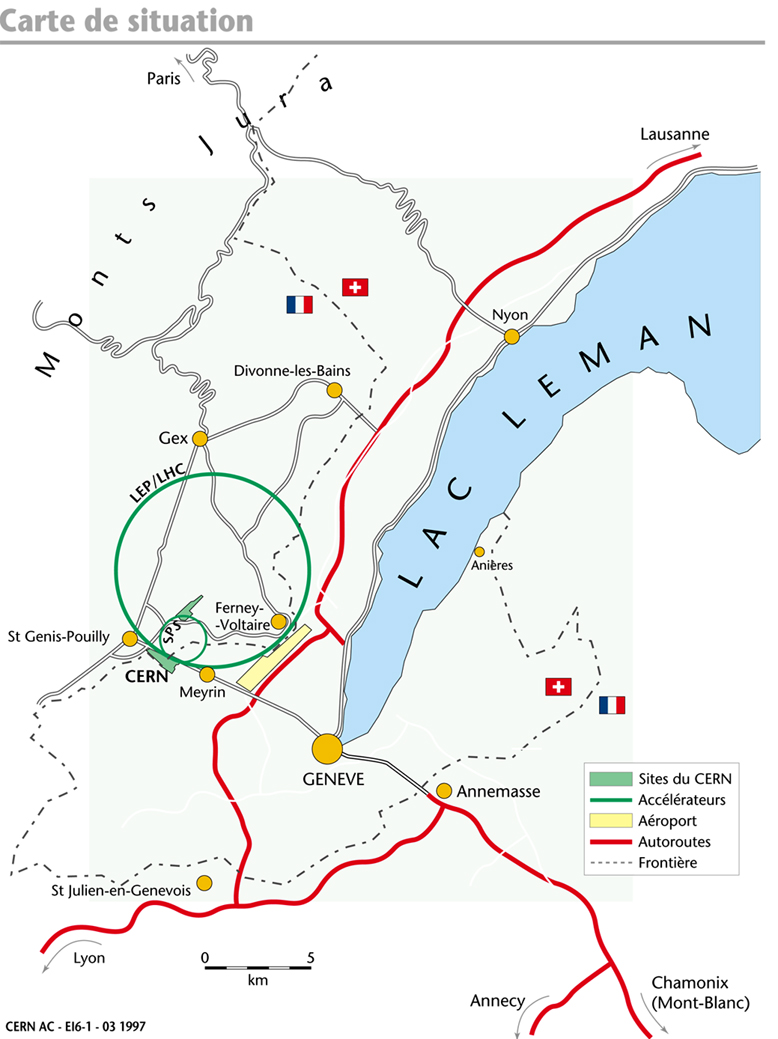
\includegraphics[width=0.35\textwidth]{Chapters/01_Introduction/Images/lhc-pho-1997-169.jpg}\\
     \caption{Map of LHC location.}
     \label{fig:LHC_map}
\end{figure}

This thesis presents an analysis based on the full proton-proton collision data from the CMS experiment in
2011 and 2012. The analysis investigates the top-antitop (\ttbar) differential cross section with respect to
some global level event variables, looking specifically at semi-leptonic \ttbar decays in the electron and
muon channels. This work was carried out in collaboration with Emyr Clement, L{}ukasz Kreczko, Sergey Senkin,
Philip Symonds under the supervision of Joel Goldstein and Greg Heath. The author's main contribution in these
studies lay in development of the C++ and Python software frameworks and scripts] used in the analyses.
Related to this, maintaining up-to-date particle object definitions, corrections, efficiencies and
prescription recommendations from working groups within CMS was a large component of the author's work. In
terms of the technical workflow employed, the author was heavily involved producing n-tuples from the
analysis-ready AOD data format, running the software to perform the prescribed analysis methods and running
final scripts on the output ROOT data to perform the final calculation and to produce results plots and
tables. Particular areas of focus regarding physics included synchronisation of the event selection and
comparison of distribution shapes between 7~\TeV and 8~\TeV data, implementing aspects of the analyses such as
selection criteria, \btagging and jet energy resolution. Also included in this thesis is a description of the
author's service work contribution to the CMS experiment, a requirement of all members of the CMS
collaboration.

Chapter~\ref{c:CMS_Detector} describes the LHC and the CMS detector, including information about the object
reconsruction process based on detector readout, to represent particles produced in collisons.
Chapter~\ref{c:the_standard_model_and_top_physics} provides an overview of the Standard Model theory and some
of its shortcomings. The main \ttbar differential cross section analysis is then covered in
Chapters~\ref{c:Differential_Cross_Section:data_simulation_and_selection},\ref{c:Differential_Cross_Section:fitting_and_unfolding}
and~\ref{c:Differential_Cross_Section:systematics_and_results}. To conclude, chapter~\ref{c:summary}
contains a summary and outlook to the future. Additional data, tables and plots are given in
Appendices~\ref{c:Appendices} and finally, the author's service work is outlined in Appendix~\ref{c:service_work}.

From the outset, natural units are used throughout this thesis, unless otherwise specifed, so that

\begin{equation}
\hbar = c = 1,
\end{equation}

meaning that mass, momentum and energy all have the same units of electronVolts (eV).